
\section{Motivation}

\begin{frame}
\frametitle{Introduction}
DNS: An approach for numerically solving
the Navier-Stokes equations
\begin{itemize}
\item Extremely fine computational grids
\item High-order accurate numerical schemes
\item e.g., \emph{compact} finite
    difference schemes for approximating derivatives
\item High computational cost
    \begin{itemize}
    \item Feasible only for simple flows
    \item Parallelism almost always required
    \end{itemize}
\end{itemize}
\end{frame}

\begin{frame}
\frametitle{Compact finite difference schemes}
A class of high-order accurate finite difference schemes
for evaluating spatial derivatives

\centering
\includegraphics[width=200px]{img/discretize-function.eps}

\begin{itemize}
\item {General form of compact schemes:
\begin{align*}
\begin{split}
f_i^{\prime} + \alpha(f^{\prime}_{i-1} + f^{\prime}_{i+1}) + \
\beta(f^{\prime}_{i-2} + f^{\prime}_{i+2}) + \hdots  = \
a\frac{f_{i+1} - f_{i-1}}{dx} + \\
b\frac{f_{i+2} - f_{i-2}}{dx} + \
c\frac{f_{i+3} - f_{i-3}}{dx} + \
    \hdots
\end{split}
\end{align*}}
\item $\alpha$, $\beta$, $a$, $b$, $\hdots$ must
    satisfy certain constraints
\item Derivative defined \emph{implicitly}
\end{itemize}
\end{frame}

\begin{frame}
\footnotesize
Solution strategy
\begin{itemize}
\item {Consider the specific scheme:
\begin{align*}
f_i^{\prime} + \frac{1}{4}(f^{\prime}_{i-1} + f^{\prime}_{i+1}) = \
\frac{3}{4}\frac{f_{i+1} - f_{i-1}}{dx}
\end{align*}}

\item {We write the expression for all points:
\begin{align*}
f_2^{\prime} + \frac{1}{4}(f^{\prime}_{1} + f^{\prime}_{3}) =
    \frac{3}{4}\frac{f_{3} - f_{1}}{dx} \\
%
f_3^{\prime} + \frac{1}{4}(f^{\prime}_{2} + f^{\prime}_{4}) =
    \frac{3}{4}\frac{f_{4} - f_{2}}{dx} \\
%
f_4^{\prime} + \frac{1}{4}(f^{\prime}_{3} + f^{\prime}_{5})
    = \frac{3}{4}\frac{f_{5} - f_{3}}{dx} \\
%
\hdots
%
f_{n-1}^{\prime} + \frac{1}{4}(f^{\prime}_{n-2} + f^{\prime}_{n})
    = \frac{3}{4}\frac{f_{n} - f_{n-2}}{dx}
\end{align*}}

\item {Special ``one-sided'' equations are needed near the boundaries:

\begin{align*}
f^{\prime}_1 + 2f^{\prime}_2 &= \frac{-5f_1 + 4f_2 + f_3}{dx} \\
%
f^{\prime}_{n} + 2f^{\prime}_{n-1}
&=
\frac{5f_{n} - 4f_{n-2} -  f_{n-1}}{dx}
\end{align*}}

\end{itemize}
\end{frame}

\begin{frame}[t]
\footnotesize
The full set of equations is expressed succinctly as:
\begin{equation*}
 \begin{bmatrix}
     1&2\\
     1/4&1&1/4\\
     &1/4&1&1/4\\
     &&1/4&1&1/4\\
     &&&1/4&1&1/4\\
     &&&&&\ddots\\
     &&&&&&\ddots\\
     &&&&&&&\ddots\\
     &&&&&&&2&1
  \end{bmatrix}
  \boxed{
  \begin{bmatrix}
      f^{\prime}_1 \\
      f^{\prime}_2 \\
      f^{\prime}_3 \\
      \vdots \\
      \vdots \\
      \vdots \\
      \vdots \\
      f^{\prime}_{n-1} \\
      f^{\prime}_n
   \end{bmatrix}
   }
 =
 \begin{bmatrix}
     \frac{-5f_1 + 4f_2 + f_3}{2dx}\\
     \frac{3(f_{3} - f_{1})}{4dx}\\
     \frac{3(f_{4} - f_{2})}{4dx}\\
     \vdots\\
     \vdots\\
     \vdots\\
     \vdots\\
     \frac{3(f_{n} - f_{n-2})}{4dx}\\
     \frac{5f_{n} - 4f_{n-1} - f_{n-2}}{2dx}
  \end{bmatrix}
\end{equation*}

Solution yields the derivatives at all points
$i=1,2, \hdots n$ simultaneously.
\begin{itemize}
\item In general, compact schemes yield banded systems
\item Tridiagonal schemes generally sufficient
\end{itemize}
\end{frame}

\begin{frame}
\frametitle{Objectives}
\begin{itemize}
    \item Exploratory work for exploiting GPUs
        in current research code
        \begin{itemize}
            \item important step for our group: Palmetto cluster
        currently has 598 GPUs (and counting)
        \end{itemize}
    \item An efficient GPU tridiagonal solver
    \item Parallelize the compact finite difference evaluation---current
        research code uses a sequential approach
\end{itemize}
\end{frame}

\begin{frame}
\frametitle{Thesis contributions}
\begin{itemize}
    \item A novel solution strategy for
        the tridiagonal systems arising in
        compact finite differences
        and other numerical schemes
    \item A strategy for evaluating compact
        finite differences on GPU-accelerated clusters
\end{itemize}
\end{frame}

